\documentclass[12pt,a4paper]{article}
\usepackage[utf8]{inputenc}
\usepackage{graphicx}
\usepackage{hyperref}
\usepackage{amsmath}
\usepackage{geometry}
\usepackage{fancyhdr}

\geometry{a4paper, margin=1in}
\graphicspath{{images/}} % Assuming your images are in the 'images' directory

\pagestyle{fancy}
\fancyhf{} % Clear header and footer
\fancyhead[L]{\leftmark} % Left header, shows the current section name
\fancyhead[R]{\thepage} % Right header, shows the page number
\fancyfoot[C]{
\includegraphics[width=2cm]{Metropolia_Logo.jpeg}} % Footer image





\begin{document}
\setlength{\parskip}{0.5em}


\begin{titlepage}
    \centering
    
\includegraphics[width=0.3\textwidth]{images/Metropolia_Logo.jpeg}\\[1cm] % Metropolia University logo
    {\large \bfseries Iot Devices and Wireless Communication\\[0.5cm]}
    {\huge\bfseries Smart Bird Feeder – Final Documentation\\[0.5cm]}
    {\large Group 5:\\
    Aaban Prasla, Abhinav Kayastha, Aleksanteri Meriläinen, Milan Thapa Magar\\
    \textit{School of ICT}\\
    \textit{Metropolia University of Applied Sciences}\\[0.5cm]}
    {\large 13 May 2024\\[1cm]}
    \vfill
    {\large Project Report}
    \vfill
\end{titlepage}

\begin{abstract}
    This report presents the development of the ‘Smart Bird Feeder’, a project undertaken by Group 5 for the "IoT Devices and Wireless Communication" course at Metropolia University of Applied Sciences. The project aimed to integrate IoT technologies to improve the functionality of a traditional bird feeder. The main objective was to design a feeder that prevents pests such as squirrels and starlings from accessing the feeder while allowing desirable birds to feed undisturbed. This involved the selection of sensors, actuators, and communication modules to create a system that operates efficiently in outdoor environments. Through the course of this project, we engaged in extensive research and design iterations to meet the defined requirements. This report outlines the group’s design process, key technologies employed, and a brief overview of the outcomes.\end{abstract}

\newpage
\tableofcontents
\newpage

\section{Introduction}
This report contains the final documentation of group 5’s Smart Birdfeeder, an IOT project developed for ‘IOT Devices and Wireless Communication’, a course at Metropolia University of Applied Science, taught by Joseph Hotchkiss. 

‘IoT-Devices and Wireless Communications’ teaches students the basics of designing an Internet connected device. In this course, students design an IoT product/system/’thing’ - from selecting individual components to sketching the operation of the software. Students study common standard wired and wireless communication protocols used to interface sensors and other devices in the system. The end device is not required to work. Instead, the focus is placed on going through the entire design process, understanding all aspects of modern IoT devices, planning and designing. The result is that students understand this process rather than build the end device.

The knowledge acquired from the lectures, course slides, and research were applied to design and develop our own IoT device which was presented during the course period in six presentations to the class. In this final project document, group 5 presents our final project: a smart bird feeder. 

\subsection{Problem Statement}
We decided to create a useful device with a simple design that would solve a real-world problem and satisfy the project requirements. As a group, we brainstormed problems that could be solved with an IoT solution and settled on a problem faced by backyard birdfeeders in North America: The common starling and grey squirrel. 

In North America, aside from the well-known birdfeeder enemy the grey squirrel, common starlings are aggressive birds that compete with native birds for nests and food which has caused significant hatred on the part of birders across the continent. 

In 1890, 100 starlings were released in New York City’s Central Park to introduce into the United States every bird mentioned in Shakespeare. In less than a century, European Starlings spread across the continent to the point where now the North American population is estimated to be over 200 million, approximately one third of the entire world’s population \cite{wbu}. 

Many pest-deterrent birdfeeders already exist on the market. However, starlings and squirrels are intelligent and agile animals that can often bypass their prevention methods and access food intended for more desirable species. The question arose of how this could be solved with an IoT solution. The group decided to turn an existing bird feeder into an internet connected device with sensors, actuators, and wired and wireless communication protocols to better deny starlings and squirrels access to food. 
\subsection{Project Overview}
To design an internet connected device, each week during the course we addressed a different aspect of the design process: 
\begin{itemize}
    \item \textbf{Initial Concept:} Here we define our problem and how our device should work to solve it.
    \item \textbf{MCU:} We research possible choices for the “brains” of our device based on predefined criteria. We narrow our choices down to four possible options and make our final decision.
    \item \textbf{Sensors and Actuators:} For our birdfeeder to operate as intended, we need to decide how our device will interact with the physical world. Here, we define our criteria for sensors and actuators and select our components.
    \item \textbf{Serial communication:} Our MCU controls the operations of our device; however, for our various components to communicate with the MCU, we must manage proper serial communication. Here we define which protocols we will use and how they work.
    \item \textbf{Wireless communication:} For the user to have remote access to the feeder (to receive data and send operation commands), we must provide a method for wireless communication. Here we explore our options and define our needs with a link budget.
    \item \textbf{PCB/schematics:} To understand how our components will share power and communicate, here we envision a rough outline of the physical design.
    \item \textbf{Software:} In this section, we present our software design, a high-level explanation of how our software will work; either RTOS or bare metal. A software flowchart aalong with class diagrams show how our main function interacts with our classes and interrupts.
\end{itemize}

The birdfeeder we chose to modify is a classic model that uses a weight sensitve levered door frame which closes when a bird or animal that is too heavy rests on the perch. This lever is adjustable by the user to allow larger or smaller birds access depending on user preferences. Starlings and squirrels are very intelligent and agile and can bypass this mechanism by either flying in place or hanging in the front. 

\begin{figure}[h]
    \centering
    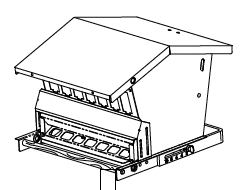
\includegraphics{images/birdhouse_drawing.png}
    \caption{Birdhouse Drawing \cite{woodlink}}
\end{figure}

We intend to modify the feeder by locking the door when it closes and remaining locked until the pest in no longer present or the user unlocks the feeder (if they chose for the feeder to remain locked before the event).

\subsection{Goals and Objectives}

The primary goal of our project is to improve the design of an existing bird feeder, enhancing its capability to prevent pests, particularly starlings and squirrels, from accessing the food.

Our objectives, which are specific and measurable actions to achieve this goal, include:
\begin{itemize}
    \item \textbf{Complete Project Requirements:} Ensure that all project specifications and requirements are met according to the course guidelines.
    \item \textbf{Documentation and Sharing:} Thoroughly document the development process and share findings with peers and course instructors.
    \item \textbf{Timely Progress:} Maintain a consistent and progressive timeline, meeting all interim milestones and deadlines.
    \item \textbf{Animal Safety:} Design the feeder in such a way that no animals are harmed, adhering to ethical considerations.
    \item \textbf{Economical and Practical Design:} Achieve a realistic, cost-effective, and simple design that can be easily implemented and maintained.
    \item \textbf{Long Battery Life:} Ensure the feeder operates efficiently with a battery life of at least six months, minimizing maintenance and recharging frequency.
\end{itemize}

\section{Requirements}
Here we outline our device requirements, including system requirements, technical specifications, and budget constraints.
\subsection{System Requirements}
The system requirements for the "Smart Bird Feeder" project are outlined in Table 1. The project's system requirements ensure functionality and user control: a locking mechanism active until pests depart, wireless communication for remote management, and a minimum six-month battery life to reduce upkeep. The design considers animal safety and environmental durability within a budget of 50€, balancing cost-effectiveness with robust performance.


\begin{table}[h]
\centering
\begin{tabular}{|p{0.3\linewidth}|p{0.6\linewidth}|}
\hline
\textbf{Requirement} & \textbf{Description} \\ \hline
Prevent Intelligent pest from bypassing lock mechanism & 
- Lock the feeder when both switches are triggered \newline
- Remain locked until pest is gone \\ \hline
Provide Cloud Communication & 
- Send event data to User \newline
- Receive lock/unlock commands \newline
- Display event history \\ \hline
Power efficiency & 
- 6 months battery life \\ \hline
Animal safe design & 
- No birds and animals should be harmed \\ \hline
Weather/Temperature Proof & 
- Able to resist harsh weather conditions like wind and rain. \newline
- Able to operate in –40-to-80-degree temperature. \\ \hline
Budget & 
- 50 € \\ \hline
\end{tabular}
\caption{System Requirements of the Smart Bird Feeder}
\label{tab:system_requirements}
\end{table}

\subsection{Technical Requirements}
The technical requirements for the "Smart Bird Feeder" project are detailed in table 2:

\begin{table}[h]
\centering
\begin{tabular}{|p{0.4\linewidth}|p{0.5\linewidth}|}
\hline
\textbf{Specification} & \textbf{Description} \\ \hline
Operating Temperature Range & -40° to 80° C \\ \hline
Bird Weight Limit & Less than 60 g \\ \hline
Presence Range & Less than 0.5 m \\ \hline
Solenoid Activation Time & Less than 35 ms \\ \hline
LoRa Communication Range & Up to 5 km \\ \hline
Waterproof/Resistant & IP67 or greater \\ \hline
\end{tabular}
\caption{Technical Requirements of the Smart Bird Feeder}
\label{tab:technical_requirements}
\end{table}

The operating temperature range of our components is between -40 to 80 C so that this device can operate across different regions. The weight of a Starling is 60 to 100 grams, therefore we set a weight limit of 60g\cite{inaturalist}. We only want to detect presence in the immediate vicinity of the feeder, therefore the presence sensor will detect presence in a range of less than 0.5 meters, ensuring effective coverage in front of the feeder. With the average reaction time of a squirrel being 39ms \cite{gatewaytoairguns}, we've determined that our actuator needs to operate faster to prevent them effectively. Consequently, we've established the solenoid activation time to be less than 35ms to ensure swift response and prevent access by squirrels. Regarding wireless communication, it is important to note that actual coverage may vary depending on the components chosen and environmental factors such as urban or rural settings. Setting a 5-kilometer range enables dependable transmission of data between the bird feeder and the user, suitable for housing yards and cottage compounds. Additionally, to protect the feeder from rain, we have opted for components with an IP67 or greater waterproof rating, ensuring operation in rainy conditions.


\section{Components}

To create our birdfeeder, a microcontroller, sensor, actuator and a wireless communication module are needed. In this section each of those components are introduced along with some additional components. 

\subsection{Microcontroller Unit}

\begin{figure}[h]
    \centering
    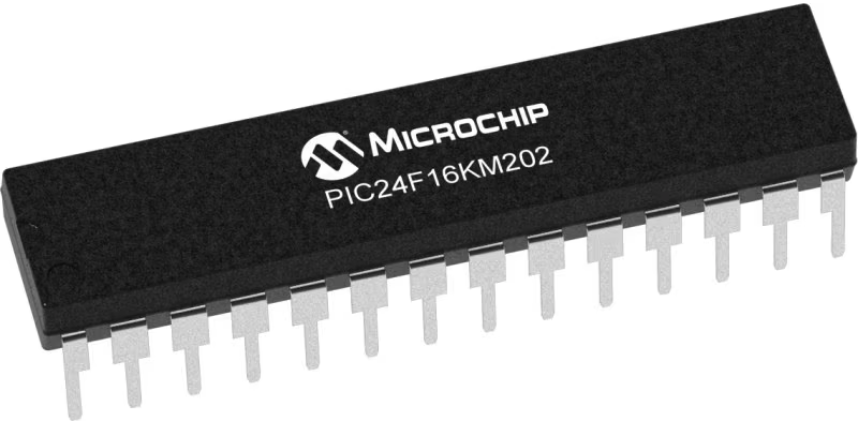
\includegraphics[width=0.5\textwidth]{images/MCU.png}
    \caption{MICROCHIP - PIC24F16KM202-I/SP \cite{mcu}}
\end{figure}

When selecting our MCU, we carefully considered various options to ensure it could accommodate any additional changes we might make to our original plan. Our priority was finding an MCU with more than enough I/O pins and support for multiple interfaces. Additionally, power efficiency was crucial, so we focused on MCUs with low operating voltage. 

Memory capacity was another key factor; we wanted enough room to program and store code without concerns about program size limitations. Furthermore, since our birdfeeder needs to operate year-round, we wanted an MCU capable of functioning across a wide range of temperatures. 

After a thorough evaluation, we chose the "MICROCHIP - PIC24F16KM202-I/SP" MCU. It met our requirements while being cost-effective, having numerous I/O pins, and supporting multiple serial communication interfaces. This choice provided the versatility and performance needed for our project. 

\begin{table}[h]
    \centering
    \begin{tabular}{|l|l|}
    \hline
    \textbf{Specification} & \textbf{Description} \\ \hline
    Price (€)              & 3.85                 \\ \hline
    Voltage                & 1.8V to 3.6V         \\ \hline
    Number of Pins         & 28                   \\ \hline
    Number of I/O's        & 24                   \\ \hline
    Interfaces             & I2C, SPI, UART, USB  \\ \hline
    Program Memory Size    & 16 KB                \\ \hline
    RAM Memory Size        & 2 KB                 \\ \hline
    Operating Temperature  & -40°C to 85°C        \\ \hline
    \end{tabular}
    \caption{MICROCHIP - PIC24F16KM202-I/SP Specifications}
    \label{tab:microchip_specs}
    \end{table}
\subsection{Sensors}
Our project required the use of at least one sensor. However, for our birdfeeder we needed two sensors; a sensor that detects when the birdfeeder’s hatch is closed and a sensor to detect the presence of the pest near the birdfeeder. 
\subsubsection{Closing Detector}

\begin{figure}[h]
    \centering
    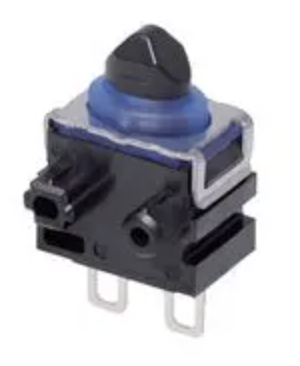
\includegraphics[width=0.25\textwidth]{images/Microswitch.png}
    \caption{Omron Microswitch - D2EW-B03H \cite{switch}}
\end{figure}

While choosing a Closing Detector, we considered various sensors such as Hall, Piezoelectric, and Infrared. Initially, we planned to choose a Piezoelectric Force Sensor since we could use the force generated by the hatch of the birdfeeder hitting the sensor to trigger it and send a signal to lock the birdfeeder. However, after further consideration, we decided against it since none of the datasheets we reviewed indicated water/weather resistance. Additionally, we were uncertain about the durability of the sensors and how they would function under constant impact from the hatch. 

We also evaluated Infrared Sensors as an option. These sensors could be installed behind the hatch, while the Infrared light is being reflected the sensor wouldn't trigger, but when the hatch closes and the light will not be reflected, the sensor would trigger sending the signal to lock the birdfeeder. However, our primary concern with this sensor was its constant transmission of Infrared Light, which we believe would drain the battery quickly, not ideal for a battery-operated device like ours. 

In the end, we opted for the 'Omron Microswitch - D2EW-B03H' for our Closing Detector. We chose this Microswitch because it is waterproof, has a compact design, and has a comprehensive datasheet. This Microswitch can be activated if force is applied from the side, which is ideal for our setup. We will install two of these Microswitches, one on each side of the birdfeeder, so that they are activated when the hatch passes over them. Since these Microswitches will be exposed to the birds, we want to ensure that birds pecking on them don't activate the Linear Actuator. To prevent this, using software we will program it so that the Linear Actuator only gets activated when both Microswitches are activated simultaneously. 

\begin{table}[h]
    \centering
    \begin{tabular}{|l|l|}
    \hline
    \textbf{Specification} & \textbf{Description} \\ \hline
    Price (€)              & 1.74                 \\ \hline
    Voltage                & 12V                  \\ \hline
    Ampere Rating          & 100 mA               \\ \hline
    Dimensions (L, W, H)   & 6.9 mm, 5.3 mm, 12.5 mm \\ \hline
    Degree of Water Protection & IP 67           \\ \hline
    Operating Temperature  & -40°C to 85°C        \\ \hline
    Operation Frequency    & 30 Operations Per Minute \\ \hline
    \end{tabular}
    \caption{Specifications of Omron Microswitch - D2EW-B03H}
    \label{tab:omron_microswitch Specification}
    \end{table}

\subsubsection{Presence Sensor}
\begin{figure}[h]
    \centering
    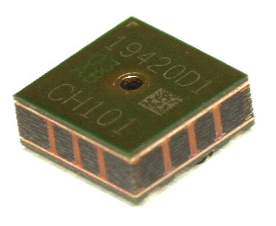
\includegraphics[width=0.25\textwidth]{images/TOF_CH101_b.png}
    \caption{TDK Ultrasonic TOF range sensor - CH101-00ABR 2 \cite{presence_sensor}}
\end{figure}
We initially considered Infrared Sensors for our Presence Sensor, having researched them previously while looking for Closing Detectors. Additionally, we also explored Ultrasonic Sensors. In comparing both options, our focus was on two key factors: the operating angle and the operating temperature. The operating angle was crucial as we aimed to cover a wide area in front of the bird feeder to ensure accurate detection, especially of pests, after locking the feeder. Operating temperature was also important, as we required our components to function reliably across a broad temperature range. 

We opted for the “TDK Ultrasonic TOF range sensor - CH101-00ABR 2” as our final choice. Our decision was  influenced by its operating angle of 180°, close range, and operating temperature. However, how we will keep it protected from the elements remains unasnwered. The sensor's compact design, low operating current, excellent datasheet and compatibility with the MCU's voltage range were additional factors in its favour. Furthermore, it utilizes the I²C Communication Protocol, which we are already familiar with. 

\begin{table}[h]
\centering
\begin{tabular}{|l|l|}
\hline
\textbf{Specification} & \textbf{Description} \\ \hline
Price (€)              & 6.85                 \\ \hline
Operating Voltage      & 1.68V to 1.98V       \\ \hline
Operating Current      & 50µA                 \\ \hline
Dimensions (L, W, H)   & 3.5mm, 3.5mm, 1.26mm \\ \hline
Operating Temperature  & -40°C to 85°C        \\ \hline
Operation Operating Angle & 180°              \\ \hline
Communication Interface & I²C                 \\ \hline
\end{tabular}
\caption{TDK Ultrasonic TOF Range Sensor - CH101-00ABR 2 Specifications}
\label{tab:tdk_sensor_specs}
\end{table}

\subsection{Actuator}
In our search for an actuator, we initially considered Servo- and Stepper-Motors. Our idea was to attach a stick to the motor's end and rotate it to secure the birdfeeder. However, we soon discovered that these options presented a few challenges: We weren't sure how much force these motors could handle, and if stepper-motors require constant power to maintain their position, which wouldn't be ideal for a battery-operated device like ours. 

Realising the limitations, we shifted our focus to Linear Actuators, which seemed more promising than Servo- and Stepper-Motors. However, all the Linear Actuators we could find in our budget were from Delta, and unfortunately, they all had the same 1-page datasheets with minimal information. 

In the end, we selected the "Delta Linear Actuator - DSTL-0216-12" due to its availability and assumed suitability for our project. While it wasn't an ideal situation, this choice provided a solution that aligned the most with our project's requirements. 

\begin{figure}[h]
    \centering
    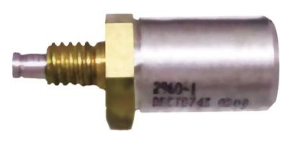
\includegraphics[width=0.4\textwidth]{images/Actuator.png}
    \caption{Delta Linear Actuator - DSTL-0216-12 \cite{actuator}}
\end{figure}

\begin{table}[h]
    \centering
    \begin{tabular}{|l|l|}
    \hline
    \textbf{Specification} & \textbf{Description} \\ \hline
    Price (€)              & 12.83                \\ \hline
    Voltage                & 12V                  \\ \hline
    Current                & 80mA                 \\ \hline
    Dimensions (Length, Diameter) & 13.2mm, 9.6mm \\ \hline
    Life Expectancy        & 100,000 Cycles Operations \\ \hline
    \end{tabular}
    \caption{Specifications of the Delta Linear Actuator - DSTL-0216-12}
    \label{tab:delta_linear_actuator_dstl_0216_12}
    \end{table}

\subsection{Wireless Communication Module}
We explored various options such as WiFi, Zigbee, and LoRa to see if they meet our wireless communication needs. To narrow down our choice, we established 2 key requirements: transmitting distance and data rate. Initially, we estimated that our device should transmit a small amount of data, up to 5 kb, over a long distance, up to 5 km. Considering these criteria, we opted for LoRa since it is a mid- to long-range wireless communication method that also meets our data rate needs. Additionally, is also has low power consumption which is great for us.

For our Wireless Communication Module, we selected the ``RF SOLUTIONS - LAMBDA68-85'' LoRa Module. We specifically chose this module because it provided the most comprehensive datasheet among the options we researched. Additionally, it has a lower receiver sensitivity and operating current.

To validate our selection and ensure it met our criteria, we performed a link budget calculation using an online tool:
\begin{itemize}
    \item Gains: 0
    \item Losses:
    \begin{itemize}
        \item Transmitter Loss: 2 dB
        \item Miscellaneous Loss: 10 dB
        \item Receiver Loss: 2 dB
        \item Open Path Loss: 105.2 dB (Distance: 5 km and Frequency: 868 MHz)
    \end{itemize}
    \item Received power formula:
    \begin{itemize}
        \item Received power (dBm) = transmitted power (14 dBm) + gains $-$ losses
        \item Received power = $-$105.2 dBm
    \end{itemize}
    \item Link Budget:
    \begin{itemize}
        \item Link Budget = Received Power $-$ Receiver Sensitivity
        \item Link Budget = $-$105.2 dBm $-$ (-120 dBm, most receivers have a lower sensitivity than this)
        \item Link Budget = 14.8 dBm
    \end{itemize}
\end{itemize}

Even in a sub-optimal scenario, our calculated link budget remains at 14.8 dBm, this shows that the signal will reliably reach its intended destination.
\begin{figure}[h]
    \centering
    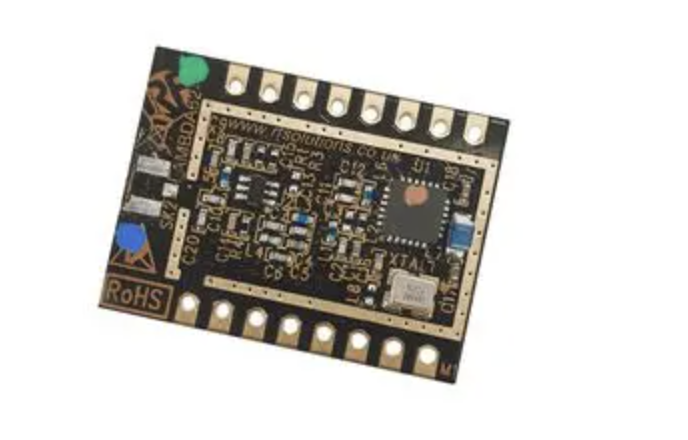
\includegraphics[width=0.5\textwidth]{images/LoRa.png}
    \caption{RF SOLUTIONS - LAMBDA68-8S \cite{lambda68}}
\end{figure}
\begin{table}[h]
    \centering
    \begin{tabular}{|l|l|}
    \hline
    \textbf{Specification} & \textbf{Description} \\ \hline
    Price (€)              & 11.66                \\ \hline
    Supply Voltage         & 1.8V to 3.7V         \\ \hline
    Operating Current      & 4.6mA (Rx), 118mA (Tx), 0.6µA (sleep) \\ \hline
    Dimensions (L, W)      & 23mm, 20mm           \\ \hline
    Operating Temperature  & -40°C to 85°C        \\ \hline
    Operation Range        & Up to 20km           \\ \hline
    Frequency              & 868/918MHz           \\ \hline
    Power Output           & 14dBm to 22dBm       \\ \hline
    Sensitivity            & Up to -148dBm        \\ \hline
    Data Rate              & 1.76 - 62.5 kbps Lora, 300kbps FSK \\ \hline
    Communication Interface & SPI                 \\ \hline
    \end{tabular}
    \caption{Specifications of the RF SOLUTIONS - LAMBDA68-8S}
    \label{tab:rf_solutions_lambda68_8s}
    \end{table}

\subsection{Additional Components}
To ensure our bird feeder circuit functions correctly with a 12V power supply, we use a voltage regulator to reduce voltage for components that require lower operating voltages. Additionally, we employ MOSFETs to manage voltage discrepancies between the higher-voltage linear actuator, microswitches, and the lower-voltage MCU.

\subsubsection{Voltage Regulator}
The Presence Sensor, MCU, and the LoRa Module operate below 12V whereas the Linear Actuator and the Microswitch operate at 12V. To ensure our components get the appropriate voltage we chose to use voltage regulator “ROHM BD9G341AEFJ-LBE2”. 

This regulator has a relatively low operating supply current and has the ideal operating temperature range, since it matches the all the other components. It can also output any voltage from 1V to 76V which covers the range that we would need, and it is also compatible with our 12V power supply since it can take any input voltage from 12V to 76V. 

The Presence Sensor, MCU, and the LoRa Module all have different operating voltage ranges, but they are all operable with 1.8V, so we have the regulator have an input voltage of 12V from our power supply and an output voltage of 1.8V. 
\begin{figure}[h]
    \centering
    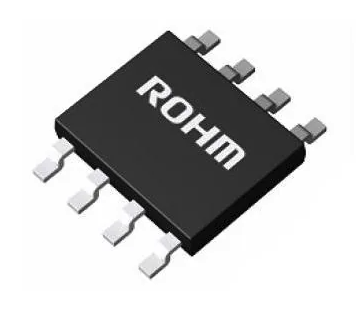
\includegraphics[width=0.4\textwidth]{images/Voltage_Reg.png}
    \caption{ROHM - BD9G341AEFJ-LBE2 \cite{voltage_regulator}}
\end{figure}

\begin{table}[h]
    \centering
    \begin{tabular}{|l|l|}
    \hline
    \textbf{Specification} & \textbf{Description} \\ \hline
    Price (€)              & 4.80                 \\ \hline
    Input Voltage          & 12V to 76V           \\ \hline
    Output Voltage         & 1V to 76V            \\ \hline
    Max Output Current     & 3A                   \\ \hline
    Operating Supply Current & 1.5mA              \\ \hline
    Operating Temperature  & -40°C to 85°C        \\ \hline
    \end{tabular}
    \caption{Specifications of the ROHM - BD9G341AEFJ-LBE2}
    \label{tab:rohm_bd9g341aefj_lbe2}
    \end{table}
\subsubsection{MOSFET}
\begin{figure}[h]
    \centering
    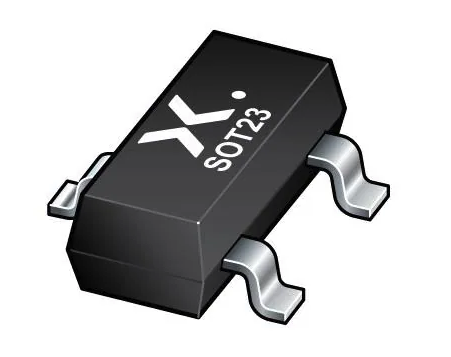
\includegraphics[width=0.25\textwidth]{images/MOSFET.png}
    \caption{Nexperia - NX7002AK,215 \cite{mosfet}}
\end{figure}
We have integrated MOSFETs in our system to manage voltage differences between the microcontroller unit (MCU), the linear actuator, and the microswitches. The selected MOSFET, Nexperia - NX7002AK,215, is chosen for its broad operating temperature range and appropriate voltage ratings (both drain-source and gate-source voltages exceed 12V), ensuring compatibility with our components.

The MCU operates at a lower voltage, which can be problematic when interfacing with higher-voltage components like microswitches. At times, signals from the microswitches may surpass the MCU's voltage capacity, causing signal loss. To mitigate this, a MOSFET reroutes power from the voltage regulator to the MCU whenever a signal from the microswitches is detected, thus preserving signal integrity.

Similarly, the lower operating voltage of the MCU is insufficient for directly controlling the linear actuator. Another MOSFET is used to bridge this voltage gap, allowing the MCU to control the actuator effectively by switching the 12V power supply as needed.
\begin{table}[h]
    \centering
    \begin{tabular}{|l|l|}
    \hline
    \textbf{Specification} & \textbf{Description} \\ \hline
    Price (€)              & 0.15                 \\ \hline
    Drain Source Voltage   & 60V                  \\ \hline
    Gate Source Voltage    & -20V to 20V          \\ \hline
    Operating Temperature  & -40°C to 85°C        \\ \hline
    \end{tabular}
    \caption{Specifications of the Nexperia - NX7002AK,215}
    \label{tab:rohm_bd9g341aefj_lbe2}
    \end{table}
\subsection{Bill of Materials (BOM)}
In our Bill of Materials, we list all our selected components, model number, manufacturer, amount used and price. Overall, our project goal was to keep our budget under 50 € which we came very close to, with a total cost of 53.19 €. 
\begin{table}[h]
    \centering
    \begin{tabular}{|l|l|l|c|r|}
    \hline
    \textbf{Name} & \textbf{Part-Model \#} & \textbf{Manufacturer} & \textbf{Amount} & \textbf{Price (€)} \\ \hline
    MCU & PIC24F16KM202 & MICROCHIP & 1 & 3.85 \\ \hline
    TOF Range Sensor & CH101-00ABR & TDK & 1 & 9.12 \\ \hline
    Switch & D2EW-B03H & OMRON & 2 & 1.74 \\ \hline
    Linear Actuator & DSTL-0216-12 & DELTA & 1 & 12.84 \\ \hline
    LoRa Module & LAMBDA68-8S & RF Solutions & 1 & 11.66 \\ \hline
    Buck Regulator & BD9G341AEFJ & ROHM & 1 & 3.53 \\ \hline
    MOSFET & NX7002AK,215 & Nexperia & 3 & 1.47 \\ \hline
    Barrel Jack & FC681465S & CLIFF  & 1 & 2.56 \\ \hline
    Actuator/Switch Conns. & XAP-02V-1 & JST & 3 & .11 \\ \hline
    Jumper & 6-09002115121 & Würth & 1 & .33 \\ \hline
    Resistors & - & - & 9 & \textasciitilde.10 \\ \hline
    Capacitors & - & - & 4 & \textasciitilde.10 \\ \hline
    \textbf{Total} & - & - & - & \textbf{53.19} \\ \hline
    \end{tabular}
    \caption{Project Bill of Materials}
    \label{tab:bom}
    \end{table}

    \section{Serial and Wireless Communication}
    \subsection{Serial Communication}
    Effective communication between the microcontroller and peripheral devices is achieved through various serial communication protocols, each selected for its specific capabilities and role within the system:
    
    \begin{itemize}
        \item \textbf{I2C (Inter-Integrated Circuit)}: This two-wire, low-speed protocol is essential for connecting and facilitating communication between multiple low-speed peripherals like sensors and secondary controllers. In our feeder, I2C is primarily used to read data from the presence sensor, which helps determine if an animal is nearby.
        \item \textbf{GPIO (General Purpose Input/Output)}: These pins are versatile for reading inputs and sending output signals directly, without complex communication protocols. In our design, GPIOs are crucial for detecting whether the feeder's hatch is open or closed, allowing the system to respond to changes in the feeder's state immediately.
        \item \textbf{SPI (Serial Peripheral Interface)}: Known for its higher data transfer rates compared to I2C, SPI is utilized for managing communications with our wireless communication module. This is vital for ensuring rapid and reliable data exchange between the feeder and the remote user interface, enhancing the responsiveness of the system to user commands and status updates.
    \end{itemize}
    

    
    \subsection{Wireless Communication}
    For wireless communication, we opted for LoRaWAN due to its long-range capabilities and low power consumption, which are ideal for outdoor applications such as the Smart Bird Feeder:
    
    \begin{itemize}
        \item \textbf{LoRa WAN}: This technology enables our bird feeder to transmit data over long distances (up to 20 km in rural areas) \cite{wikipedia_lora}, making it suitable for remote monitoring. It allows the feeder to send real-time notifications and status updates to the user, and receive remote commands to lock or unlock the feeder mechanism.
    \end{itemize}
    
\section{Implementation}
\subsection{Block Diagram}
\begin{figure}[h]
    \centering
    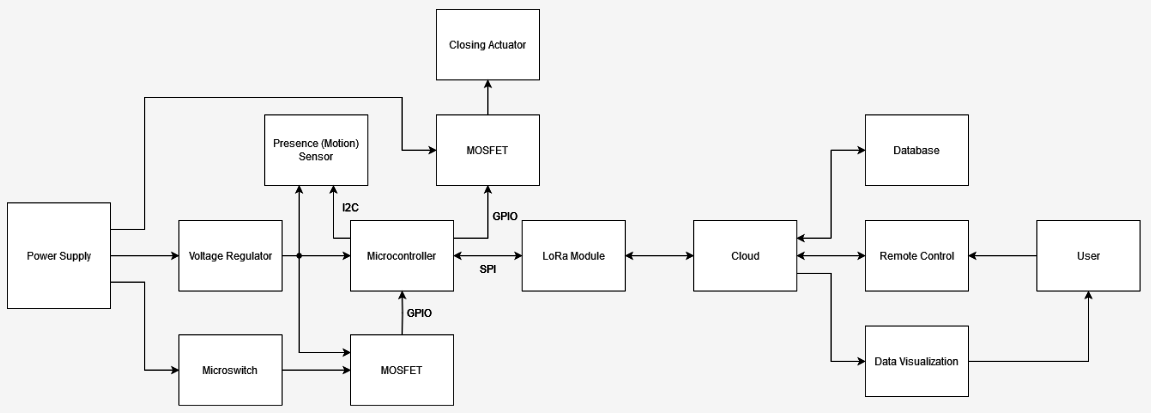
\includegraphics[width=1\textwidth]{images/Block_Diagram.png}
    \caption{Block Diagram of the Smart Bird Feeder}
\end{figure}


This block diagram aims to show the overall design of the bird feeder, sensors and actuator usage, data collection, transmission of the data and the overall user experience. The system is powered by a 12V battery connected to a voltage regulator that steps down the voltage to 1.8V for the microcontroller and presence sensor.  

Communication between the microcontroller and the presence sensor is achieved using the I2C protocol for the efficient transmission of data. The use of the presence sensor is critical as it signals to the microcontroller to unlock the locked door if no motion from pests is detected within a predetermined interval. The microswitch communicates with the microcontroller via GPIO, which determines the state of the door (closed or open) and indicate to activate the actuator.  

Controlling the power and adapting the signal between the high voltage and low voltage components are done using MOSFETs, where the microswitch’s high unnecessary voltage is grounded so the microcontroller can safely receive the signal from the microswitch. For the closing actuator the microcontroller sends a signal to a MOSFET which drives the closing actuator. 

The system’s ability to communicate over long distances and perform remote operations is achieved by a LoRa module using the SPI communication protocol. This module allows for the microcontroller to connect to the cloud for transfer of data and allow for user interaction (user commands). The cloud plays a critical role to handle data storage, event logging and enabling user interaction in the form of remote control and data visualization. 
\subsection{Physical Design}
To complete the initial physical design of our device, the group used KiCad, a free software suite used for electronic design automation (EDA) that facilitates the design and simulation of electronic hardware for printed circuit board (PCB) manufacturing \cite. 

With KiCad and information from each selected component’s datasheet, we were able to simulate the wiring and power management and render a 3D representation of our device’s PCB. 

This proved to be a complex process as it was the first time we had used this software. Our results are not yet functional but instead represent a hypothetical design based on our current abilities and what we have learned so far in the course and education. 
\subsubsection{Schematics}
Below are the schematics for the PCB (fig 9.), MCU (fig.10), Solenoid, Power Supply, Voltage Regulator (fig. 11), and Switch (fig. 12).
\begin{figure}[h]
    \centering
    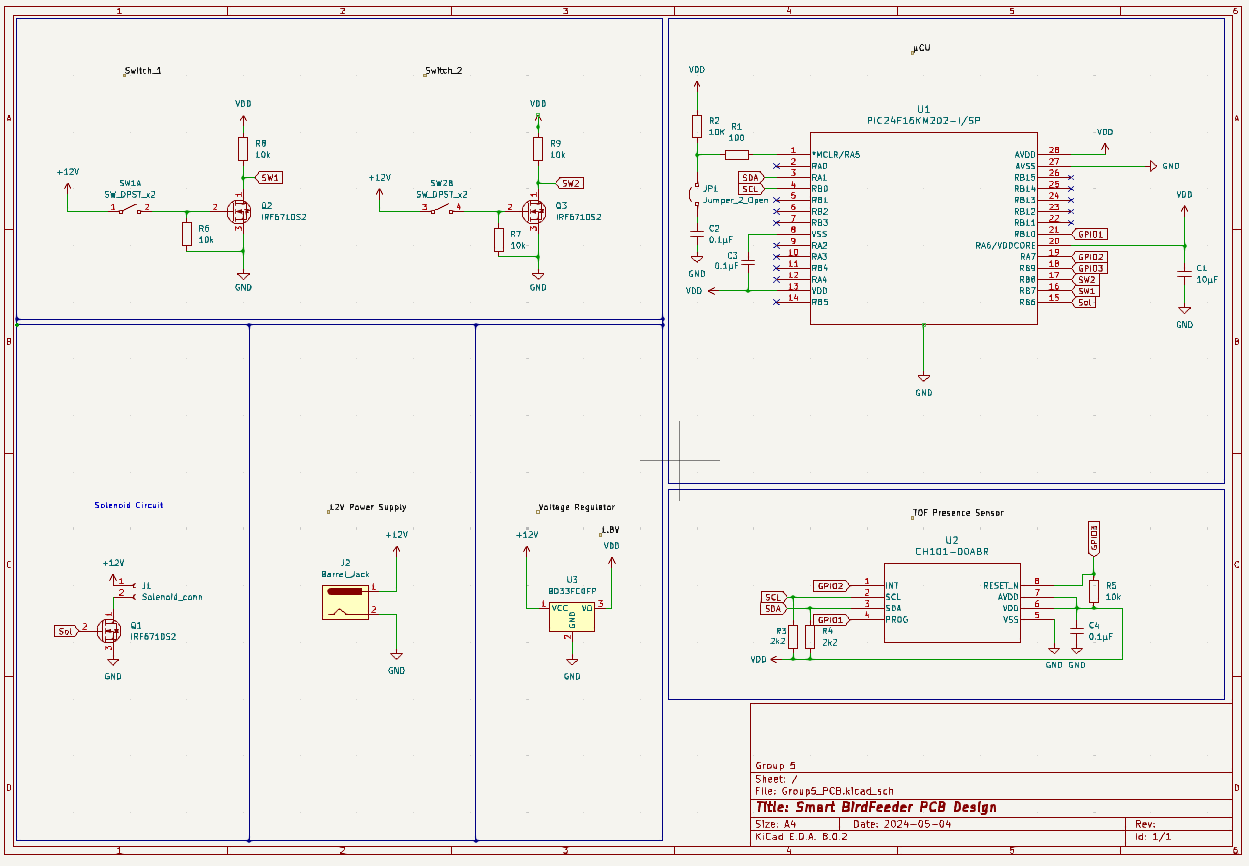
\includegraphics[width=.75\textwidth]{images/BirdFeeder_Schematics.png}
    \caption{PCB Schematics displaying all components/connections}
\end{figure}
\begin{figure}[h]
    \centering
    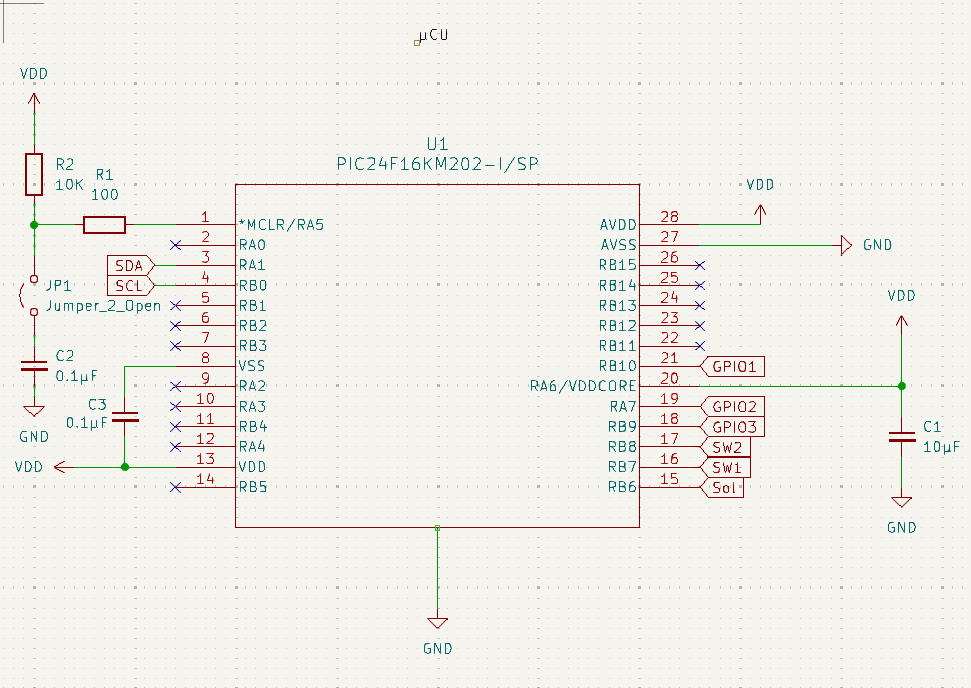
\includegraphics[width=.75\textwidth]{images/MCU_Schematics.png}
    \caption{MCU Schematics displaying connections}
\end{figure}
\begin{figure}[h]
    \centering
    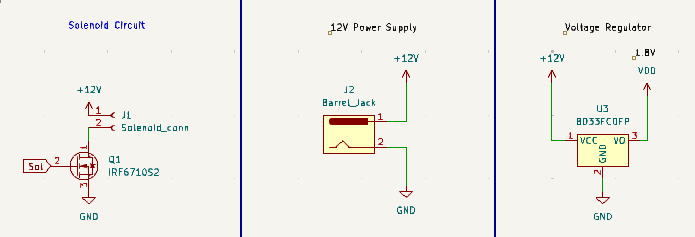
\includegraphics[width=.75\textwidth]{images/Solenoid_12VPower_VReg_Schematics.png}
    \caption{Solenoid, Power Supply, and Voltage Regulator Circuits Schematics}
\end{figure}
\begin{figure}[h]
    \centering
    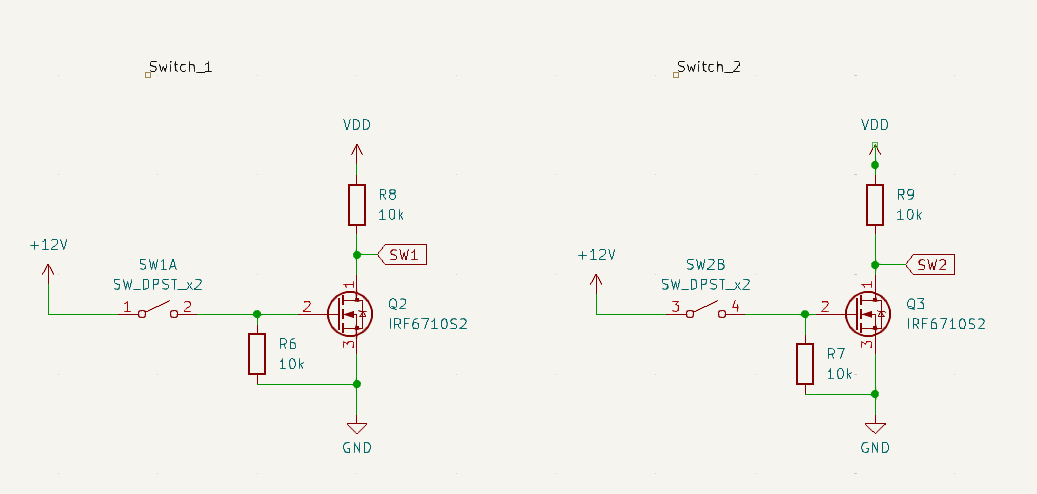
\includegraphics[width=.75\textwidth]{images/Switch_schematics.png}
    \caption{Switch Circuit Schematics}
\end{figure}
\subsubsection{PCB 3D Render}
Using KiCad, the footprint (fig.14) and 3D rendering (fig. 13) of the PCB was created to visualize the physical design of the bird feeder. The foot print and 3D rendering provides a clear representation of the components, their placement, and the overall layout of the PCB.
\begin{figure}[h]
    \centering
    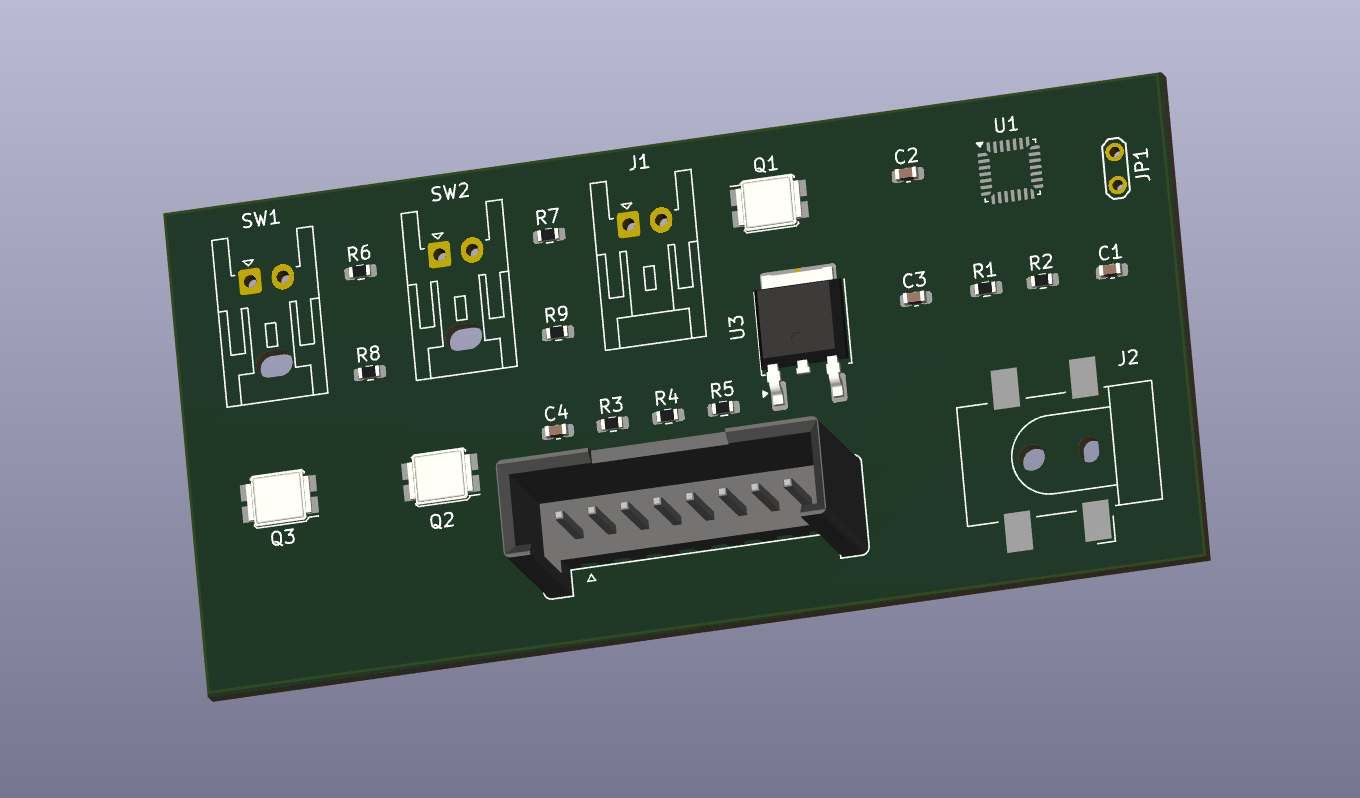
\includegraphics[width=.75\textwidth]{images/PCB_3D.png}
    \caption{3D PCB Rendering}
\end{figure}
\begin{figure}[h]
    \centering
    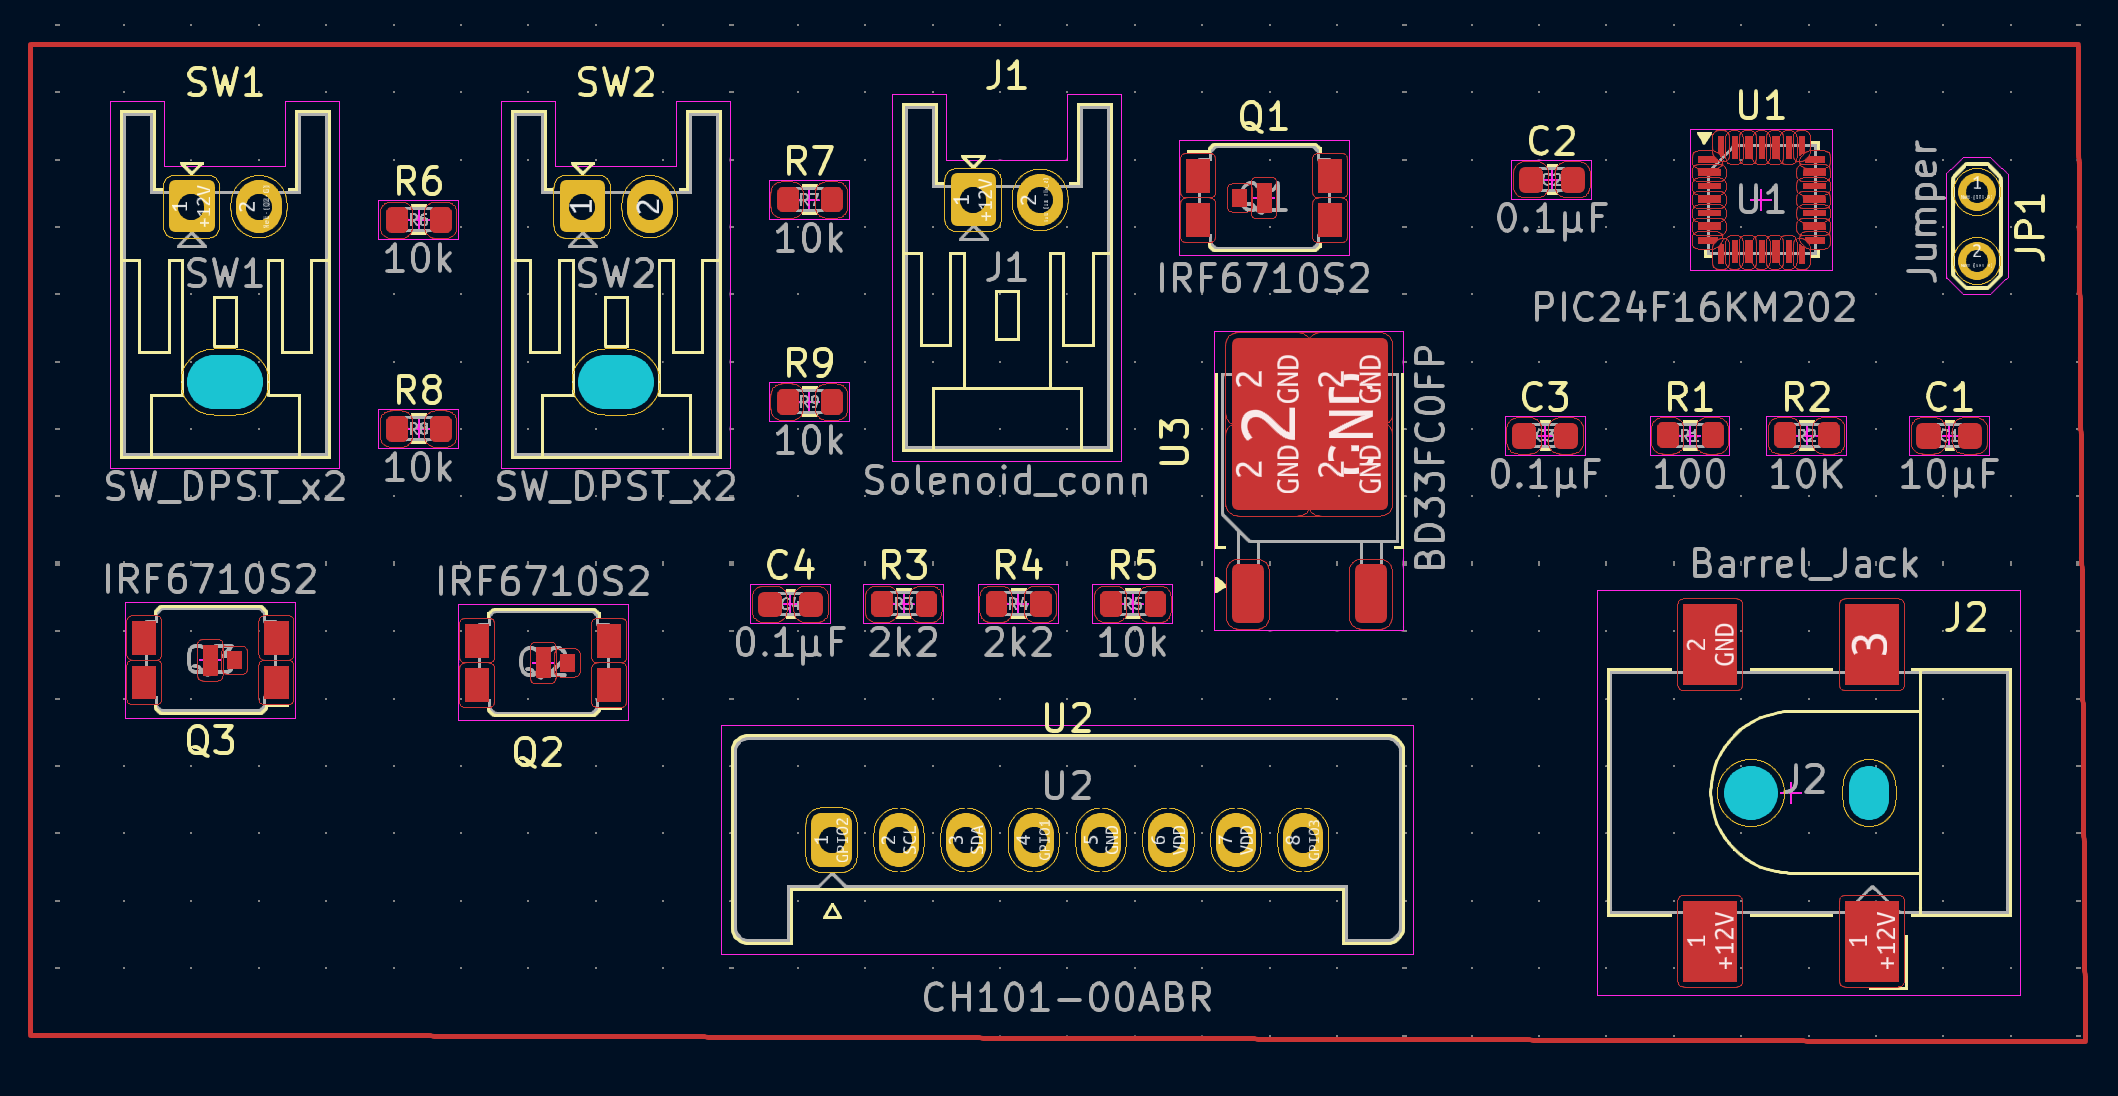
\includegraphics[width=.5\textwidth]{images/PCB_Footprint.png}
    \caption{PCB Footprint with labelled components}
\end{figure}
\subsection{Software}
\subsection{Bare-metal vs RTOS}
While selecting between Bare-Metal and RTOS for managing tasks and resources it is important to look at both and see which one fits the specific requirements of our birdfeeder the best. Bare-Metal systems directly interact with hardware without the abstraction layer of an operating system, executing code and offering efficiency. Conversely, RTOS provides task scheduling and multitasking capabilities, enabling deterministic timing and easier real-time task management. 

As we don't have real-time constraints we decided to go with a Bare-Metal system. Additionally, the simplicity of Bare-Metal systems will allow us to easily debug any problems we may face while coding the birdfeeder, contributing to overall reliability. 
\subsubsection{Class Diagram}

The class diagram (fig. 16) shows the structure of our system, including the classes, their attributes, and the methods they will use. The main classes are the \texttt{Event\_Handler} class, which will be responsible for the overall functionality of the birdfeeder, and the \texttt{Wireless\_Communication\_Handler} class, which will be responsible for the user interface and communication with the cloud.

\begin{figure}[h]
    \centering
    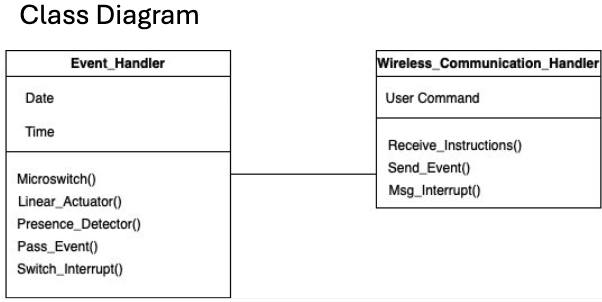
\includegraphics[width=1\textwidth]{images/class_diagram.png}
    \caption{class diagram}
\end{figure}
\subsubsection{Flowchart}

\begin{figure}[h]
    \centering
    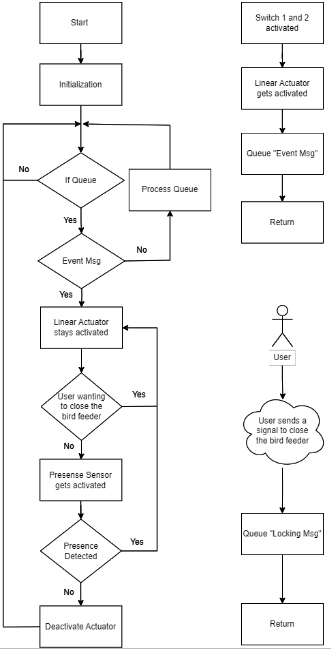
\includegraphics[width=0.5\textwidth]{images/flowchart.png}
    \caption{Software Flowchart}
\end{figure}

In figure 17, we can see a Flowchart depicting how our system functions. We have a main loop and 2 interrupts, in our main loop, we will implement a queue that will check if there are any new messages from the interrupts.  

“Interrupt 1” will be responsible for the case when both Microswitches are triggered, it will activate the Linear Actuator and send an “Event Msg” message to the queue in the main loop. “Interrupt 2” will be responsible for the case when the user sends a “User Msg” message to the queue in the main loop.  

Going back to the main loop, based on which interrupt is triggered and what message is received in the queue, the main loop will execute some code. It will check whether the message is an “Event Msg”, if it is not then the only other message will be the “User Msg”, in this case, the program will “Process Queue”, meaning store the information in the message and then clear the queue and continue checking if there are any new messages. If the message is an “Event Msg” the program will keep the Linear Actuator activated and check if the user wants to close the birdfeeder based on whether the program has received a “User Msg”. If there is no “User Msg” the program will check whether the pest is still present using the Presence Sensor and after the pest has left the program will deactivate the Linear Actuator thus opening the birdfeeder and will return to checking if any new messages arrived in the queue. Alternatively, while checking if the user wants to close the birdfeeder if there is a “User Msg” then the program will keep the birdfeeder and return to checking if any new messages arrived in the queue, and in this case, the birdfeeder will be unlocked only when the main receives another "User Msg" message or the birdfeeder runs out of battery. 
\subsubsection{UI/UX}

\begin{figure}[h]
    \centering
    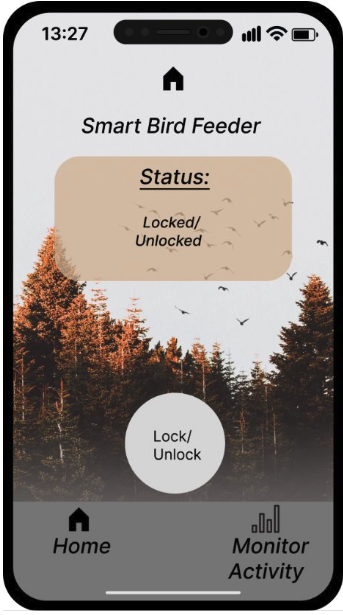
\includegraphics[width=0.5\textwidth]{images/UI_Home.png}
    \caption{User Interface - Home Screen}
\end{figure}

\begin{figure}[h]
    \centering
    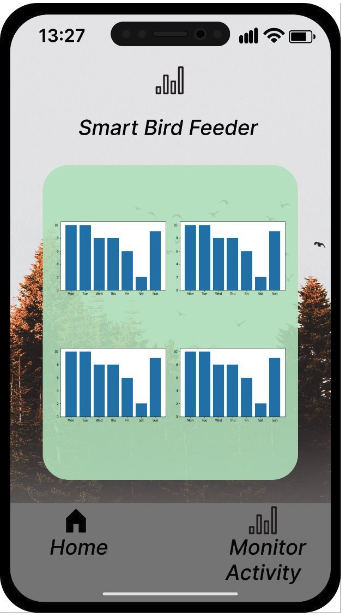
\includegraphics[width=0.5\textwidth]{images/UI_Data.png}
    \caption{User Interface - Data Screen}
\end{figure}

Below, Figures 18 and 19 are a visual representation of what kind of a user interface we may have. In our design the user will be shown which page they are in, whether it is the "Home” page or the “Monitor Activity” page, with an icon near the top of the page. 

If the user is on the “Home” page they will see the status of the birdfeeder at this moment, whether it is locked or unlocked. Below the Status they will see a button which they can press to either lock or unlock the birdfeeder and below that the user will see the navigation bar where they can choose to go between the “Home” page or “Monitor Activity” page. 

If the user is on the “Monitor Activity” page they will see 4 graphs, each showing the number of times the birdfeeder has closed within a specific time period. The graph on the top left showing weekly activity, top right showing monthly activity, bottom left showing activity in the last 6 months and the bottom right graph showing annual activity. The user can press each graph to maximise it and press the “Monitor Activity” button on the navigation bar to return to watch all 4 activity graphs. 
\section{Conclusion}
The Smart Bird Feeder project successfully met most of the initial technical and system requirements, despite challenges like inadequate datasheets and budget constraints. Our focus on pest prevention and efficient operation led to selecting reliable components suitable for varying environmental conditions. While not all envisioned features were implemented, the project significantly enhanced our understanding of IoT development and set a strong foundation for future enhancements.

\subsection{Requirements Achieved}

In our bird feeder, we aimed to meet all the system and technical needs. Most parts met our expectations, but some may not deliver as desired because the datasheet lacks enough information. The information below displays our requirements and whether they are met:

\begin{itemize}
    \item \textbf{Pest Prevention:} The bird house model includes a mechanical lever adjustable to close the door based on weight, with a maximum weight limit set at 60g to exclude heavier pests.
    
    \item \textbf{Temperature Range:} All selected components, including sensors, are capable of operating within a wide temperature range from -40° to 80°, except for the linear actuator, for which temperature functionality is undetermined due to insufficient datasheet information.
    
    \item \textbf{Presence Detection Range:} The presence sensor activates after the door is locked, detecting pest presence for 20 seconds, with a detection range of up to 0.5m, utilizing a sensor capable of covering up to 1.2m and 180° wide angle.
    
    \item \textbf{Solenoid Activation Time:} We have configured the solenoid activation time to be less than 35ms. However, due to insufficient information provided in the datasheet, we are unable to confirm its functionality.
    
    \item \textbf{Waterproof:} All components, except for the microswitches, will be hidden inside the compartment. Microswitches located on the door's edge are water-resistant with IP67 ratings, meeting environmental exposure requirements.
    
    \item \textbf{Wireless communication:} Our device employs LoRaWAN technology, offering a range of up to 20 km, exceeding our need of 5 km for sending event data to and receiving lock/unlock commands from users.
    
    \item \textbf{Animal Friendly Design:} Our aim is to make the bird feeder animal-friendly so that it does not harm any pest that comes around the feeder. Since we are upgrading the existing model without changing any of its mechanical operations, we believe our smart feeder will be animal-friendly.
    
    \item \textbf{Power Efficiency:} To save power, we employ software interrupts, allowing the device to sleep when inactive and only awaken when triggered by a switch or user command.
    
    \item \textbf{Budget:} Although the total cost is slightly above our initial budget of 50 €, it remains within an acceptable range at 53.90€.
\end{itemize}
\subsection{Challenges}

During the course, the group faced many challenges, which are detailed below:

\begin{itemize}
    \item \textbf{Unsatisfactory Datasheets:}
    Datasheets with limited information and insufficient details about components led the group to discard many options, as there was no assurance that these components would meet the project's criteria.
    
    \item \textbf{Budgeting Issues:}
    High-quality components often did not fit within the group's budget or project criteria. This necessitated extended research into alternative implementations and sourcing components from different suppliers.
    
    \item \textbf{Refining Bird Feeder Idea:}
    The initial project scope included ambitious features such as bird identification through a camera. However, further research revealed that these features were not feasible, as they overcomplicated the design. Consequently, the focus was shifted to the core functionality of the bird feeder—preventing pests and undesirable animals from accessing the feed.
    
    \item \textbf{Lack of Power Management Calculations:}
    Without precise data on the system's power consumption, the group could not confidently guarantee a battery life of six months. More detailed power consumption data would also help identify any components using unnecessarily high power, which could then be optimized or replaced.
    
    \item \textbf{PCB Design:}
    The design of the PCB and schematics posed significant challenges, primarily due to the team's limited experience with PCB design and the use of KiCad software. This aspect of the project required substantial learning and adaptation.
\end{itemize}

\section{References}
\begin{thebibliography}{9}
    \bibitem{inaturalist}
    European Starling (California Academy of Sciences Living Roof Fauna) ·  iNaturalist. (n.d.). iNaturalist. 
    \url{https://www.inaturalist.org/guide_taxa/473960}
    
    \bibitem{gatewaytoairguns}
    Squirrel Reaction Times? - Airguns \& Guns Forum. (n.d.).
    \url{https://www.gatewaytoairguns.org/GTA/index.php?topic=78406.0}
    
    \bibitem{woodlink}
    Woodlink. (n.d.). Retrieved May 13, 2024, from \url{https://www.woodlink.com/}
    
    \bibitem{ipratings}
    Waterproof ratings: Ingress Protection (IP) ratings. (n.d.). 
    \url{https://www.iec.ch/ip-ratings}
    
    \bibitem{kicad}
    Wikipedia contributors. (2024a, April 8). KiCad. Wikipedia. 
    \url{https://en.wikipedia.org/wiki/KiCad}
    
    \bibitem{wbu}
    Starling facts: Wild Birds Unlimited - Nature Shop. (n.d.-b). 
    \url{https://eugene.wbu.com/european-starling}
    
    \bibitem{mcu}
    MCU: PIC24F16KM202. (n.d.). Microchip. 
    \url{https://www.microchip.com/en-us/product/pic24f16km202}
    
    \bibitem{presence_sensor}
    Presence Sensor: CH101 | TDK InvenSense. (2023, August 7). TDK InvenSense. 
    \url{https://invensense.tdk.com/products/ch101/}
    
    \bibitem{switch}
    Switch: Omron-Electronics/D2EW-B03H. (n.d.). Mouser Electronics. 
    \url{https://www.mouser.com/ProductDetail/Omron-Electronics/D2EW-B03H}
    
    \bibitem{actuator}
    Actuator: Delta-Electronics/DSTL-0216-12. (n.d.). Mouser Electronics.
    \url{https://www.mouser.com/ProductDetail/Delta-Electronics/DSTL-0216-12}
    
    \bibitem{lambda68}
    LoRa transceiver Module: LAMBDA68 - RF 868MHz, SURFACE MOUNT, 20KM+ RANGE. (n.d.). Radio Modules From RF Solutions UK. 
    \url{https://www.rfsolutions.co.uk/radio-modules-c10/lambda68-rf-lora-transceiver-module-868mhz-surface-mount-20km-range-p972}

    \bibitem{voltage_regulator}
    Voltage Regulator: ROHM-Semiconductor/BD9G341AEFJ-LBE2. (n.d.). Mouser Electronics.
    \url{https://www.mouser.com/ProductDetail/ROHM-Semiconductor/BD9G341AEFJ-LBE2}
    
    \bibitem{mosfet}
    MOSFET: Infineon IRFH5210 DataSheet. (n.d.). Infineon Technologies. 
    \url{https://www.infineon.com/dgdl/Infineon-IRFH5210-DataSheet-v01_01-EN.pdf}

    \bibitem{wikipedia_lora}
    Wikipedia contributors. (2024c, May 6). LoRa. \textit{Wikipedia}. Available online: \url{https://en.wikipedia.org/wiki/LoRa}

\end{thebibliography}

    

\end{document}
